\documentclass{beamer}
\usepackage{pgfpages}
%\usepackage[utf8]{inputenc}
\usepackage{times}
\usepackage{tikz}
\usetheme[titlepagelogo=images/logo,
	color=blue,
	language=english,
	bullet=triangle,
	secondsupervisor=false,
	assistantsupervisor=false,
	secondassistantsupervisor=false,
	secondcandidate=false
]{TorinoTh}
\linespread{1.5}
\setbeamercovered{transparent}
%\usecolortheme{seahorse}
\useoutertheme{infolines}
\setbeamertemplate{footline} [frame number]
\author{LE Van Linh}
\rel{Marie BEURTON-AIMAR}
%\titlegraphic{
\includegraphics[height=0.25\paperheight]{images/logo}}
\title{Automatic morphology: landmarks estimation in biological images}
\ateneo{UNIVERSITY OF BORDEAUX}
%\author[LE Van Linh]{
%	\begin{tabular}{l r}
%	Student: & Supervisor:\\[0.2cm]
%	\textbf{LE} Van Linh & Marie \textbf{BEURTON-AIMAR}
%	\end{tabular}
%}
%\institute{LaBRI laboratory}
\date{\today}
\begin{document}
\titlepageframe

\begin{frame}{Contents}
	\tableofcontents
\end{frame}
%%%%%%%%%%%%%%%%%%%%%%%%%%%%%%%%%%%%%%%%%%%%%%%%%%%%%%%%%%%%%%%%%%%%%%%%%%%%%%
\section{Introduction}
\subsection{LaBRI laboratory}
\begin{frame}{LaBRI}
	\begin{block}{LaBRI}
		\textbf{LaBRI}\footnote{http://www.labri.fr/} is a research unit associated with the CNRS, the University of Bordeaux and the Bordeaux INP.\\[0.2cm]
		\textbf{Missions}: research, technology application and transfer and training.
	\end{block}
	\begin{block}{Staffs}
		\begin{itemize}
			\item 150 teaching/research staff
			\item 22 administrative and technical
			\item More than 140 doctoral student and post-docs.
		\end{itemize}
	\end{block}
\end{frame}
%%%%%%%%%%%%%%%%%%%%%%%%%%%%%%%%%%%%%%%%%%%%%%%%%%%%%%%%%%%%%%%%%%%%%%%%%%%%%%
\subsection{The internship}
\begin{frame}{Introduction}
	\begin{itemize}
		\item A collaborative project between LaBRI and INRA Rennes
		\item Objectives: tracking, collecting and classifying the insects based on morphometry.
		\item Programming of automatic identification of landmarks in  biological images:
			\begin{itemize}
				\item Cross-correlation
				\item Implementation based on article \textit{``\color{red}{Automatic identification of landmarks in digital images}" $^{\footnote{Palaniswamy, Sasirekha, Neil A. Thacker, and Christian Peter Klingenberg. \textbf{``Automatic identification of landmarks in digital images."} IET Computer Vision 4.4 (2010): 247-260.}}$ }
			\end{itemize} 		  
	\end{itemize}
\end{frame}
%%%%%%%%%%%%%%%%%%%%%%%%%%%%%%%%%%%%%%%%%%%%%%%%%%%%%%%%%%%%%%%%%%%%%%%%%%%%%%
\section{Method}
\subsection{Cross-Correlation}                                                              
\begin{frame}{Cross-Correlation method}
	\begin{itemize}
		\item Estimate the presentation of a template in an image.
		\item Formula:
			\begin{center}
				\begin{equation}\label{eq:cross-correlation}
					R_{ccorr}(x,y) = \sum\limits_{x',y'}[T(x'.y').I(x + x', y + y')]
				\end{equation}
			\end{center}
			\begin{itemize}
				\item \textbf{T}: template, $(x', y')$ is coordinate in template
				\item \textbf{I}: image, $(x + x', y + y')$ is coordinate on image, where we get the value to compute while template \textit{T} sliding.
			\end{itemize}
	\end{itemize}
\end{frame}
%%%%%%%%%%%%%%%%%%%%%%%%%%%%%%%%%%%%%%%%%%%%%%%%%%%%%%%%%%%%%%%%%%%%%%%%%%%%%%
\iffalse
\begin{frame}{Cross-Correlation}
	\begin{columns}[c]
		\column{0.3\textwidth}
		\begin{figure}
		
\begin{tikzpicture}
			\draw[step=1cm,gray,very thin] (-2,-2) grid (2,2);
		\end{tikzpicture}
	\end{figure}
		\column{0.3\textwidth}
		\begin{figure}
		
\begin{tikzpicture}
			\draw[step=1cm,red,very thin] (3,0) grid (5,2);
		\end{tikzpicture}
	\end{figure}
		\column{0.3\textwidth}
		\begin{figure}
		
\begin{tikzpicture}
			\draw[step=1cm,gray,very thin] (6,-2) grid (10,2);
			\draw[step=1cm,red,very thin] (6,0) grid (8,2);
		\end{tikzpicture}
		\end{figure}
	\end{columns}
\end{frame}
\fi
%%%%%%%%%%%%%%%%%%%%%%%%%%%%%%%%%%%%%%%%%%%%%%%%%%%%%%%%%%%%%%%%%%%%%%%%%%%%%%
\subsection{Edge extraction}
\begin{frame}{Edge extraction method}
	\begin{itemize}
	\item The implementation based on \textbf{"Automatic identification of landmarks in digital images"}, \textit{Palaniswamy, Sasirekha, Neil A. Thacker, and Christian Peter Klingenberg} \\
	\item It includes four steps:
		\begin{center}
			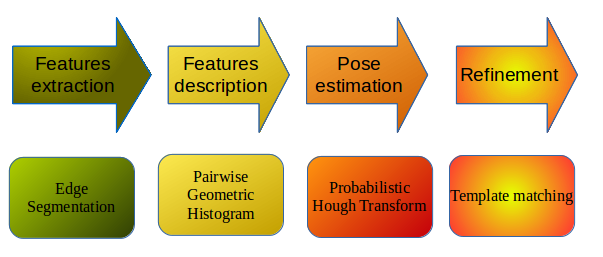
\includegraphics[height=3.5cm]{images/flow_step.png}	
		\end{center}
	\end{itemize}
\end{frame}
%%%%%%%%%%%%%%%%%%%%%%%%%%%%%%%%%%%%%%%%%%%%%%%%%%%%%%%%%%%%%%%%%%%%%%%%%%%%%%
\begin{frame}{Method - Edge segmentation}
	Purpose: 
	\begin{itemize}
		\item Extract the features (edge) from images
		\item Get the approximate segment lines
	\end{itemize}
	Method:
	\begin{itemize}
		\item Indicate the threshold value by analysis histogram of image		
		\item Canny algorithm
		\item Break edge algorithm$^{\footnote{Thacker, Neil A., P. A. Riocreux, and R. B. Yates. \textit{``Assessing the completeness properties of pairwise geometric histograms."} Image and Vision Computing 13.5 (1995): 423-429.}}$
	\end{itemize}
\end{frame}
%%%%%%%%%%%%%%%%%%%%%%%%%%%%%%%%%%%%%%%%%%%%%%%%%%%%%%%%%%%%%%%%%%%%%%%%%%%%%%
\begin{frame}{Method - Edge segmentation}
	\begin{columns}[c]
		\column{0.5\textwidth}
		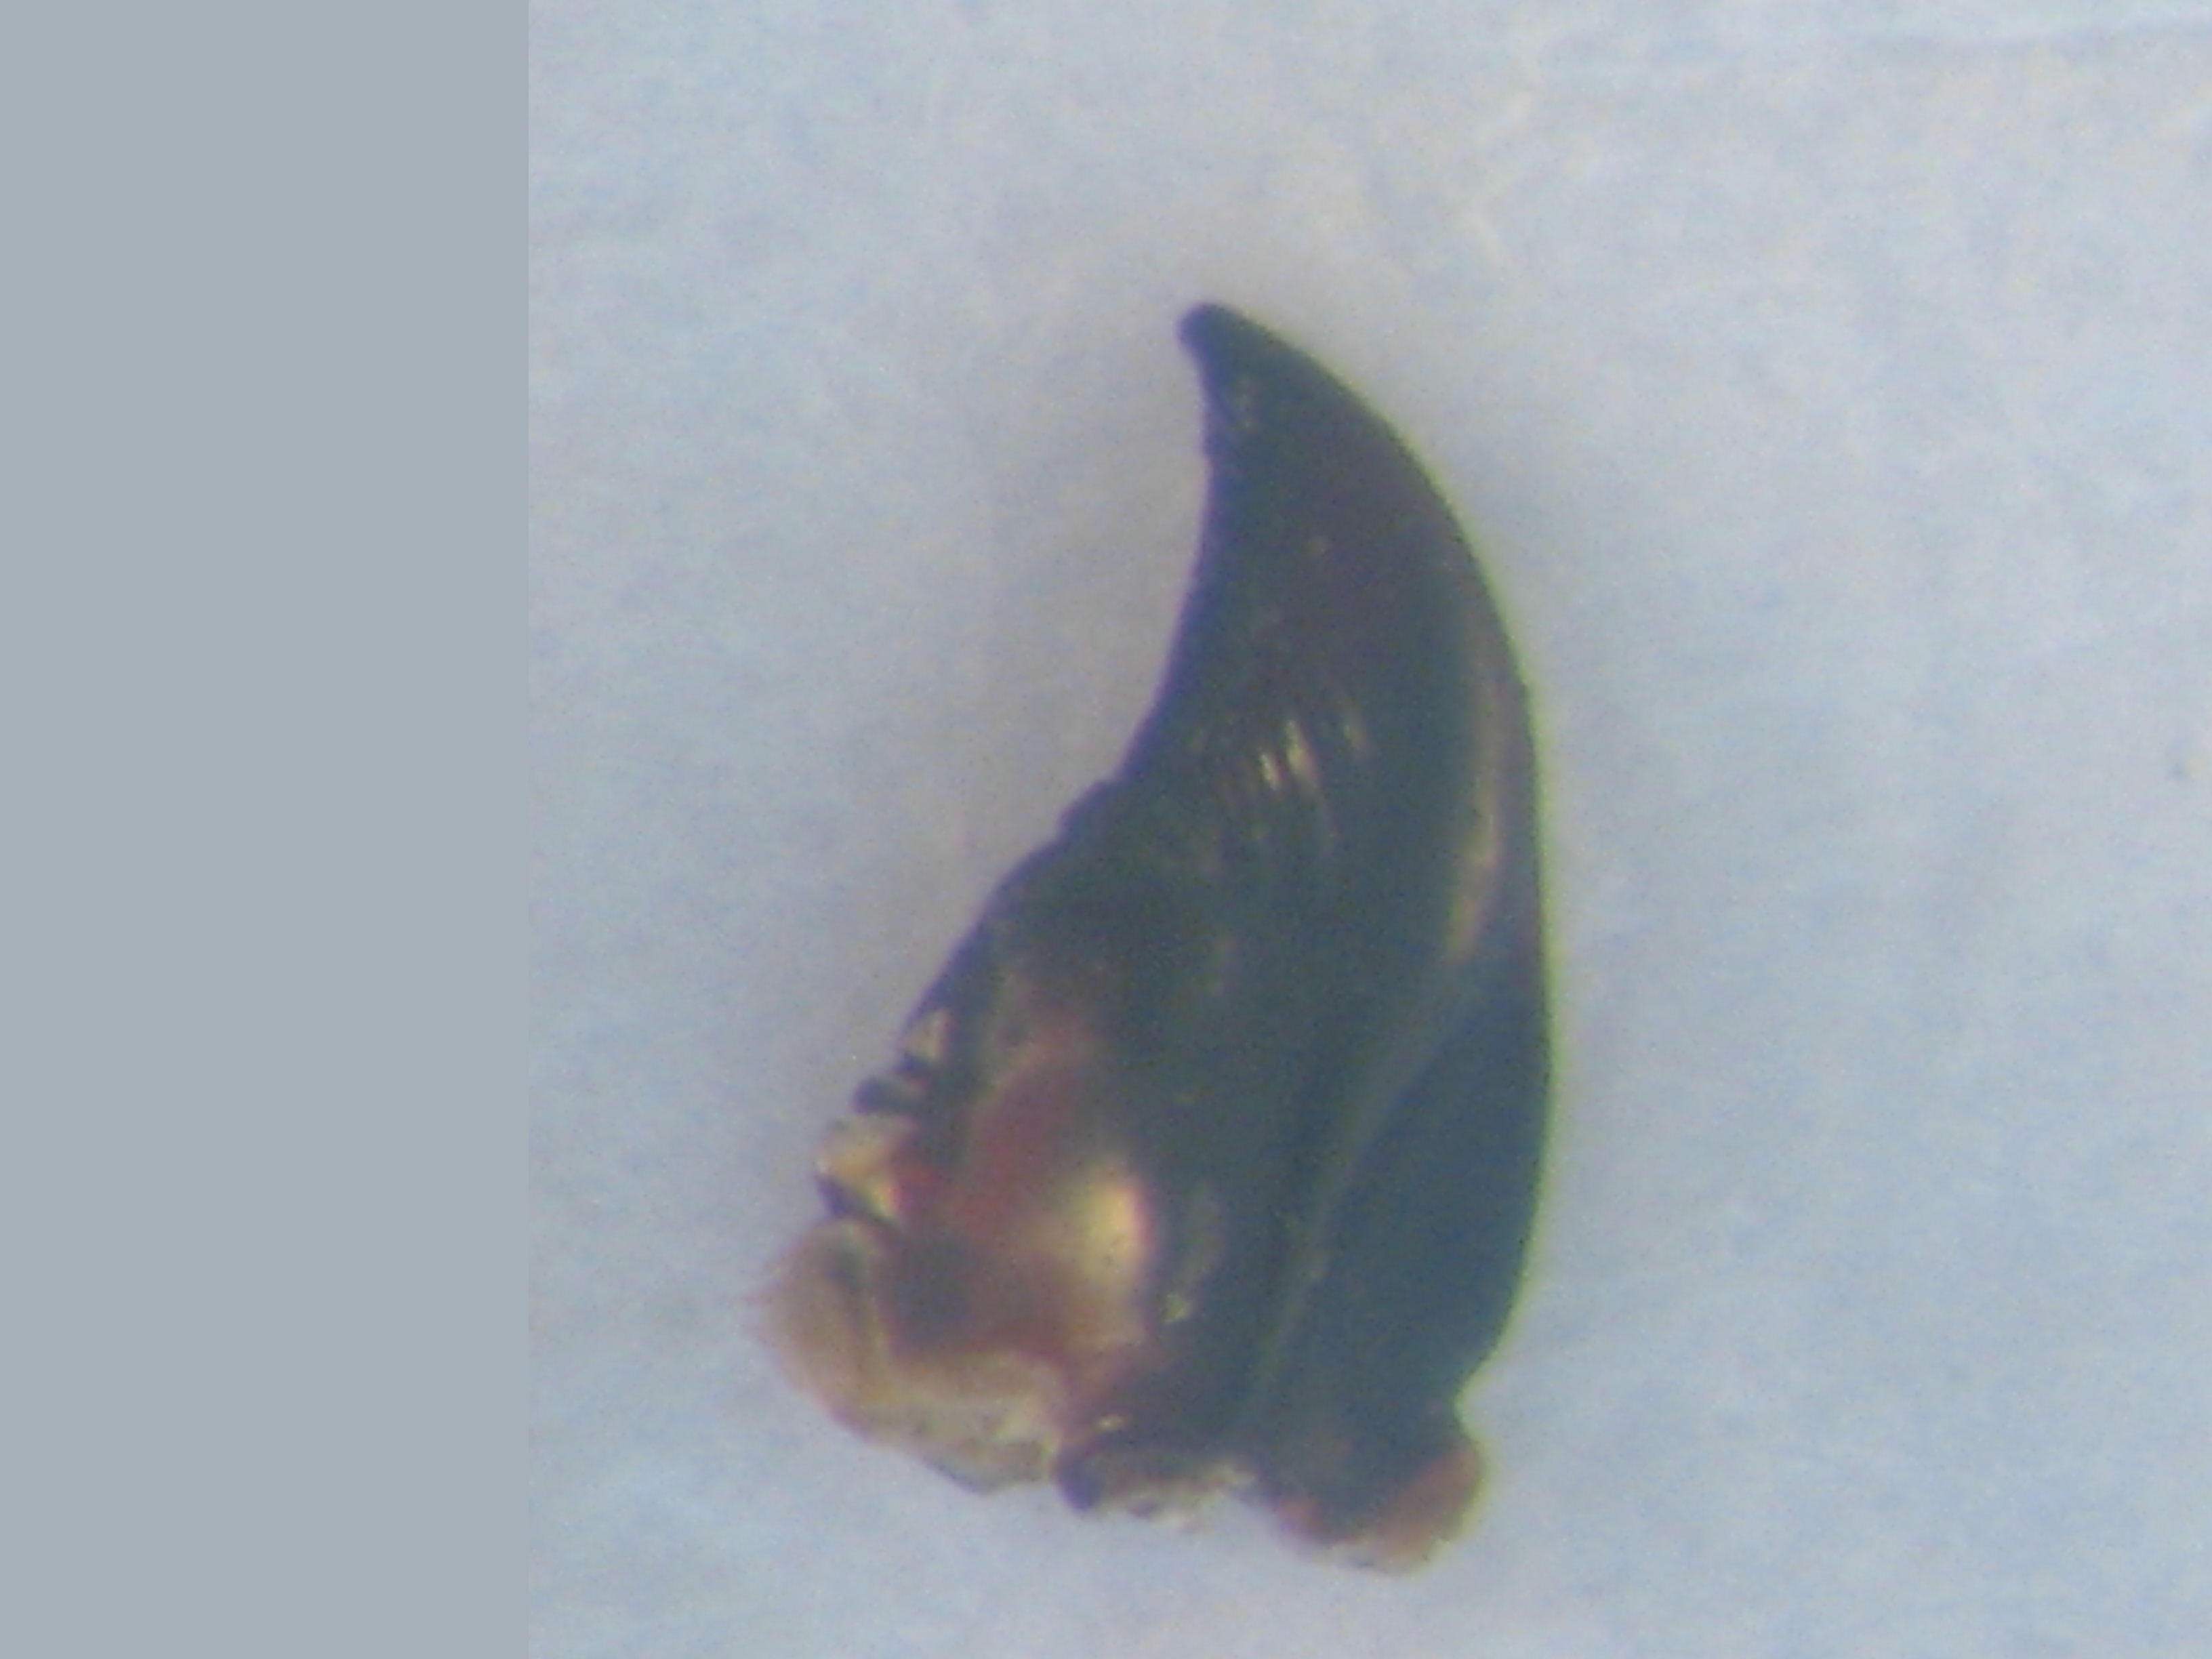
\includegraphics[height=4.5cm]{images/model28.JPG}
		\column{0.5\textwidth}
		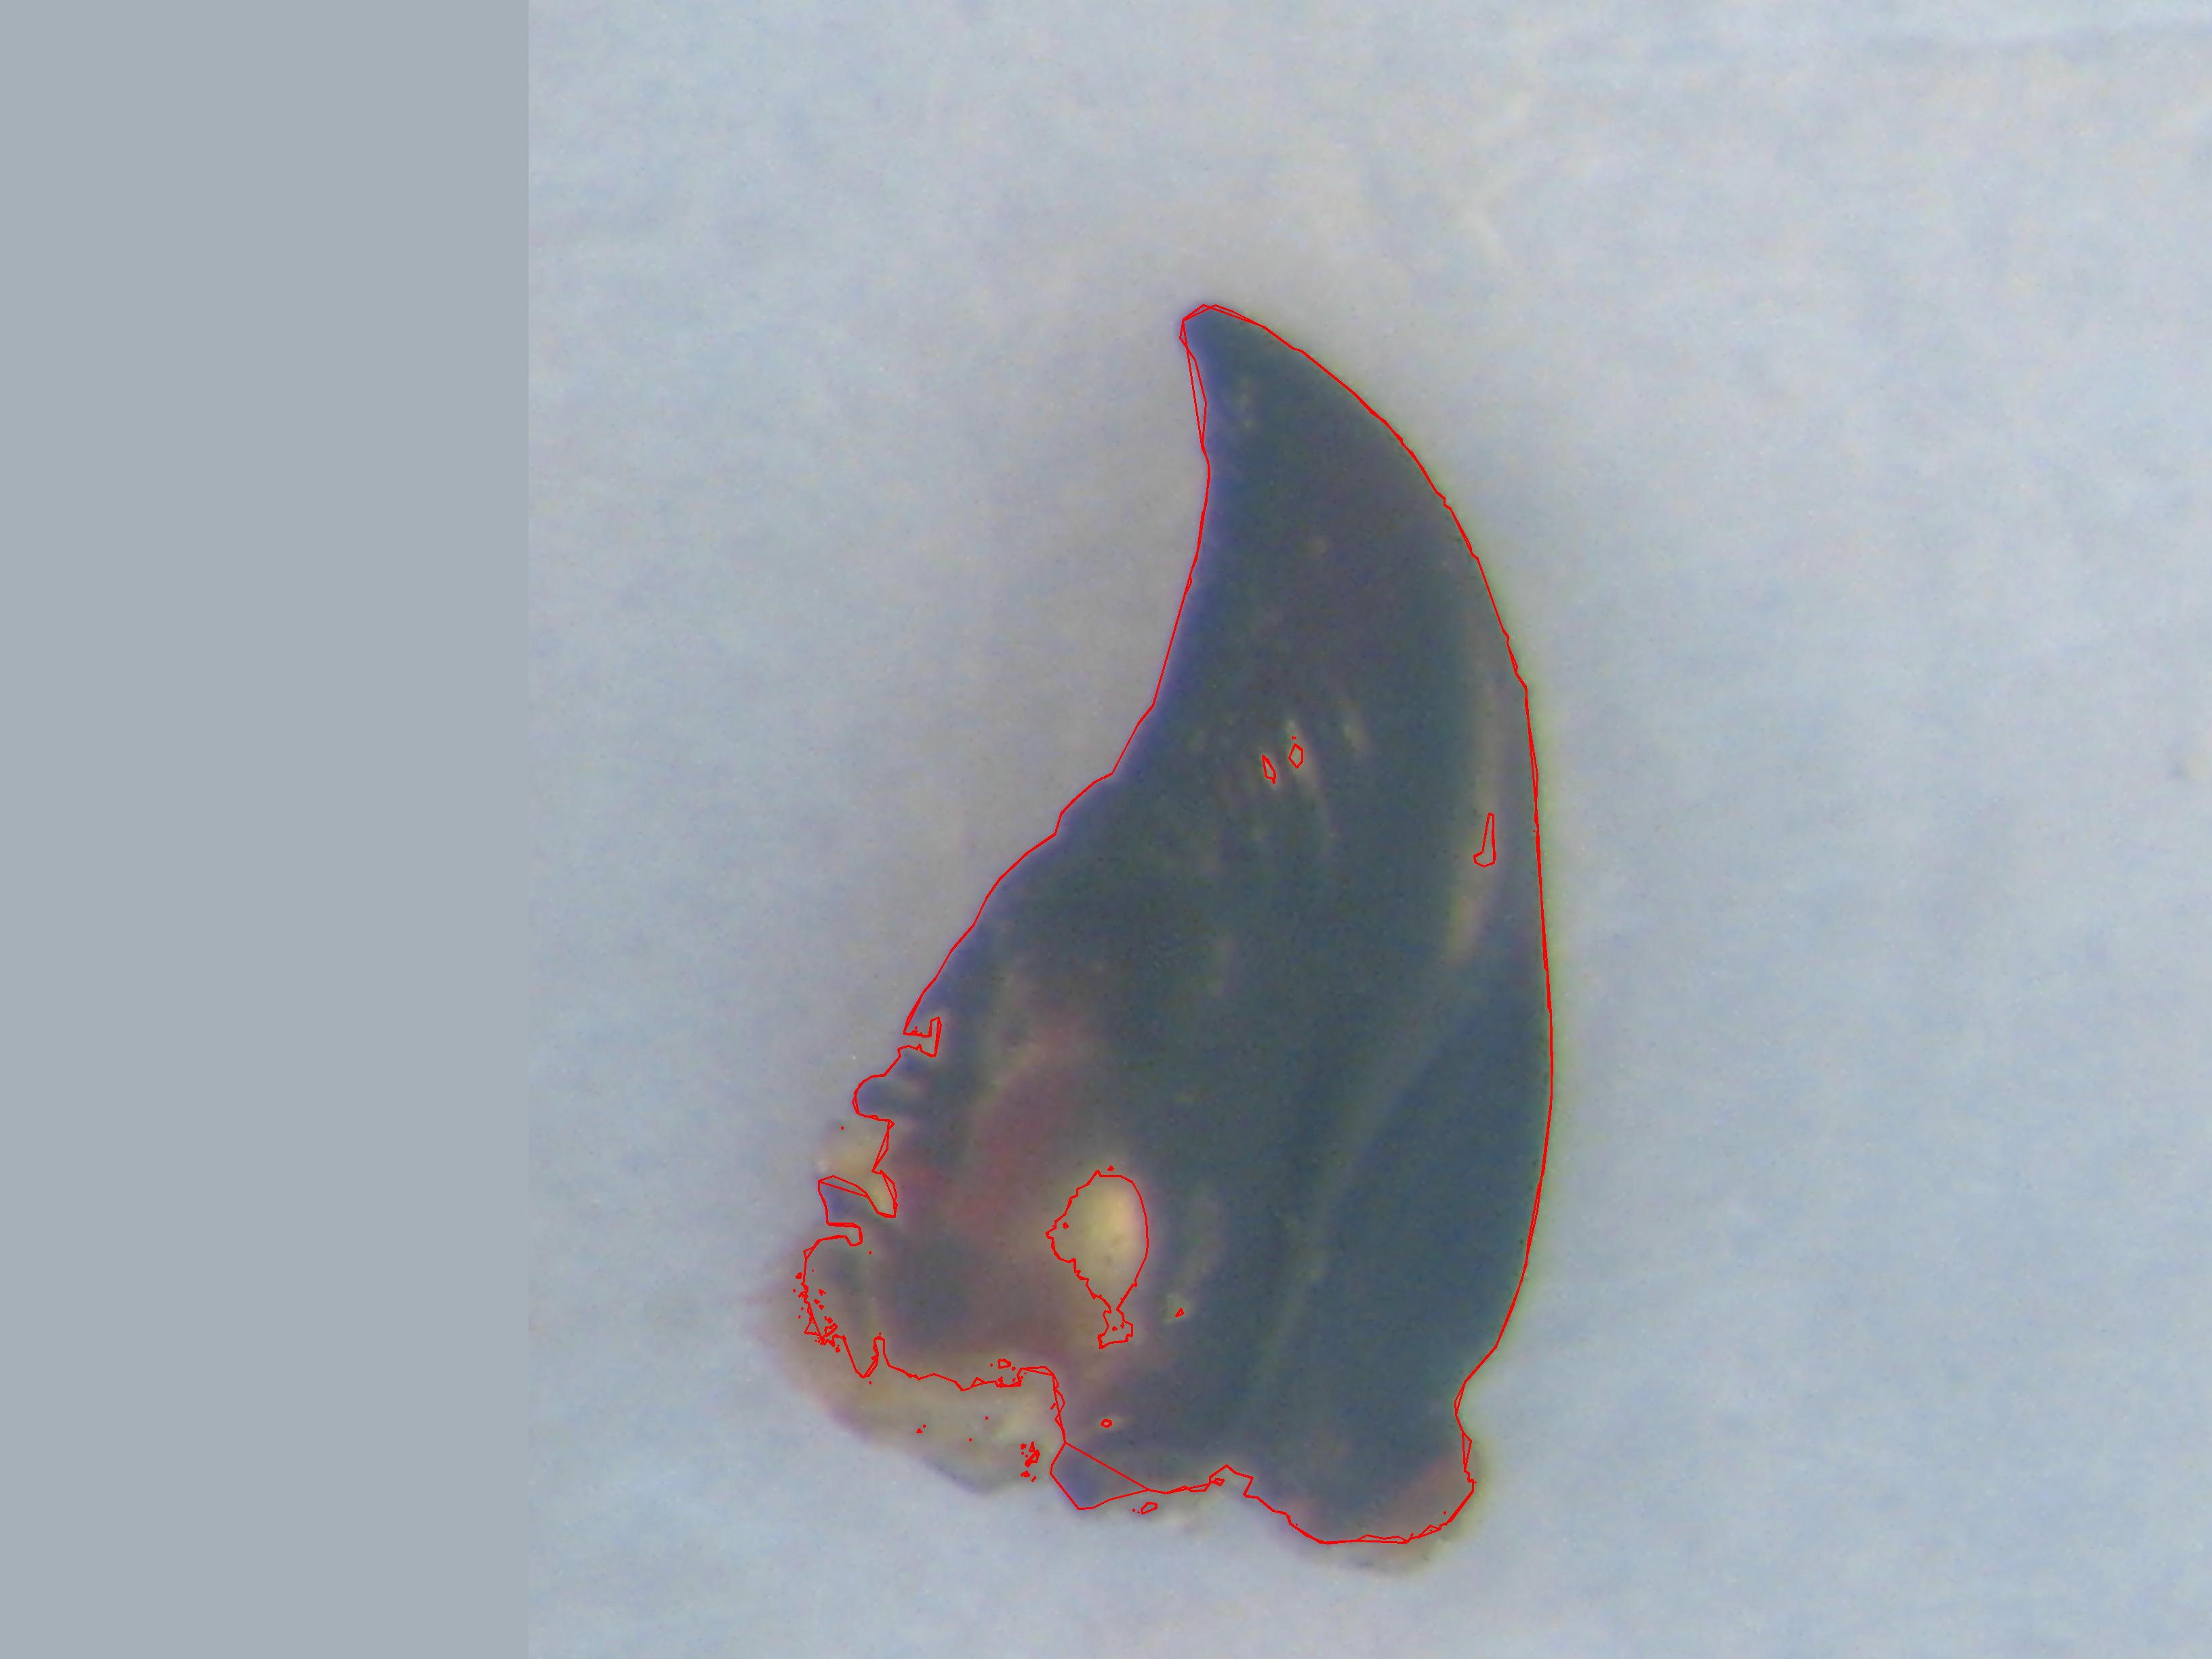
\includegraphics[height=4.5cm]{images/edge28.jpg}
	\end{columns}
\end{frame}
%%%%%%%%%%%%%%%%%%%%%%%%%%%%%%%%%%%%%%%%%%%%%%%%%%%%%%%%%%%%%%%%%%%%%%%%%%%%%%
\begin{frame}{Method - Pairwise geometric histogram}
	\begin{description}
		\item[Purpose:] detecting the present of scene image in model image
		\item[Method$^{\footnote{Thacker, Neil A., P. A. Riocreux, and R. B. Yates. \textit{``Assessing the completeness properties of pairwise geometric histograms."} Image and Vision Computing 13.5 (1995): 423-429.}}$:]
		\begin{itemize}
			\item Construct the \textbf{local PGH} for each line
			\item Construct the \textbf{shape PGH}, it is a set of local PGH
			\item Matching shape's PGH by Bhattacharyya metric
		\end{itemize}
		\item[PGH information:] angle between two lines and perpendicular distance from two endpoints of scene line to reference line.
	\end{description}
\end{frame}
%%%%%%%%%%%%%%%%%%%%%%%%%%%%%%%%%%%%%%%%%%%%%%%%%%%%%%%%%%%%%%%%%%%%%%%%%%%%%%
\begin{frame}{Method - Probabilistic Hough Transform}
	\begin{description}
		\item[Purpose:]
			\begin{itemize}
				\item Determine the presence and location of model image in scene image
				\item Estimate the landmarks in the scene image
			\end{itemize}
		\item[Method:]
		\begin{itemize}
			\item Build the reference table
			\item Find the pair of scene lines have the best ``vote" with pair of model lines
			\item Estimate the ``reference point" in scene image
			\item Estimate the landmarks
		\end{itemize}
		%\item[Result:] Estimated model landmarks on scene image
	\end{description}
\end{frame}
%%%%%%%%%%%%%%%%%%%%%%%%%%%%%%%%%%%%%%%%%%%%%%%%%%%%%%%%%%%%%%%%%%%%%%%%%%%%%%
\begin{frame}{Method - PHT parameters (Building the reference table)}
	\begin{enumerate}
		\item Choose an arbitrary \textbf{reference point}
		\item Compute the \textbf{perpendicular distance and angle} from each closet pair of model lines to \textit{reference point}.
	\end{enumerate}
	Example:
	\begin{center}
		\begin{tabular}{|c|c|c|}
		\hline
			Pair lines & space 1 & space 2 \\ \hline
			(\textcolor{red}{l1},\textcolor{blue}{l2}) & (\textcolor{red}{30;110.33}) & (\textcolor{blue}{23.5; 855})  \\ \hline
			(\textcolor{red}{l1},\textcolor{green}{l3}) & (\textcolor{red}{15; 121.5}) & (\textcolor{green}{5.5; 200})   \\ \hline
		\end{tabular}
	\end{center}
\end{frame}
%%%%%%%%%%%%%%%%%%%%%%%%%%%%%%%%%%%%%%%%%%%%%%%%%%%%%%%%%%%%%%%%%%%%%%%%%%%%%%
\begin{frame}{Method - PHT Parameters (Estimate the reference point in scene image)}
	The process to find the best vote are followed:
	\begin{itemize}
		\item Create an accumulator
		\item Find the pair of model line reasonable agreement about the \textbf{position, orientation and scale} and have the best ``vote"
		\item Estimate the reference point in scene image\footnote{Ashbrook, Anthony, et al. ``\textbf{Robust Recognition of Scaled Shapes Using Pairwise Geometric Histograms.}" BMVC. Vol. 95. 1995.}
	\end{itemize}

\end{frame}
%%%%%%%%%%%%%%%%%%%%%%%%%%%%%%%%%%%%%%%%%%%%%%%%%%%%%%%%%%%%%%%%%%%%%%%%%%%%%%
\begin{frame}{Method - Probabilistic Hough Transform}
	\begin{center}
		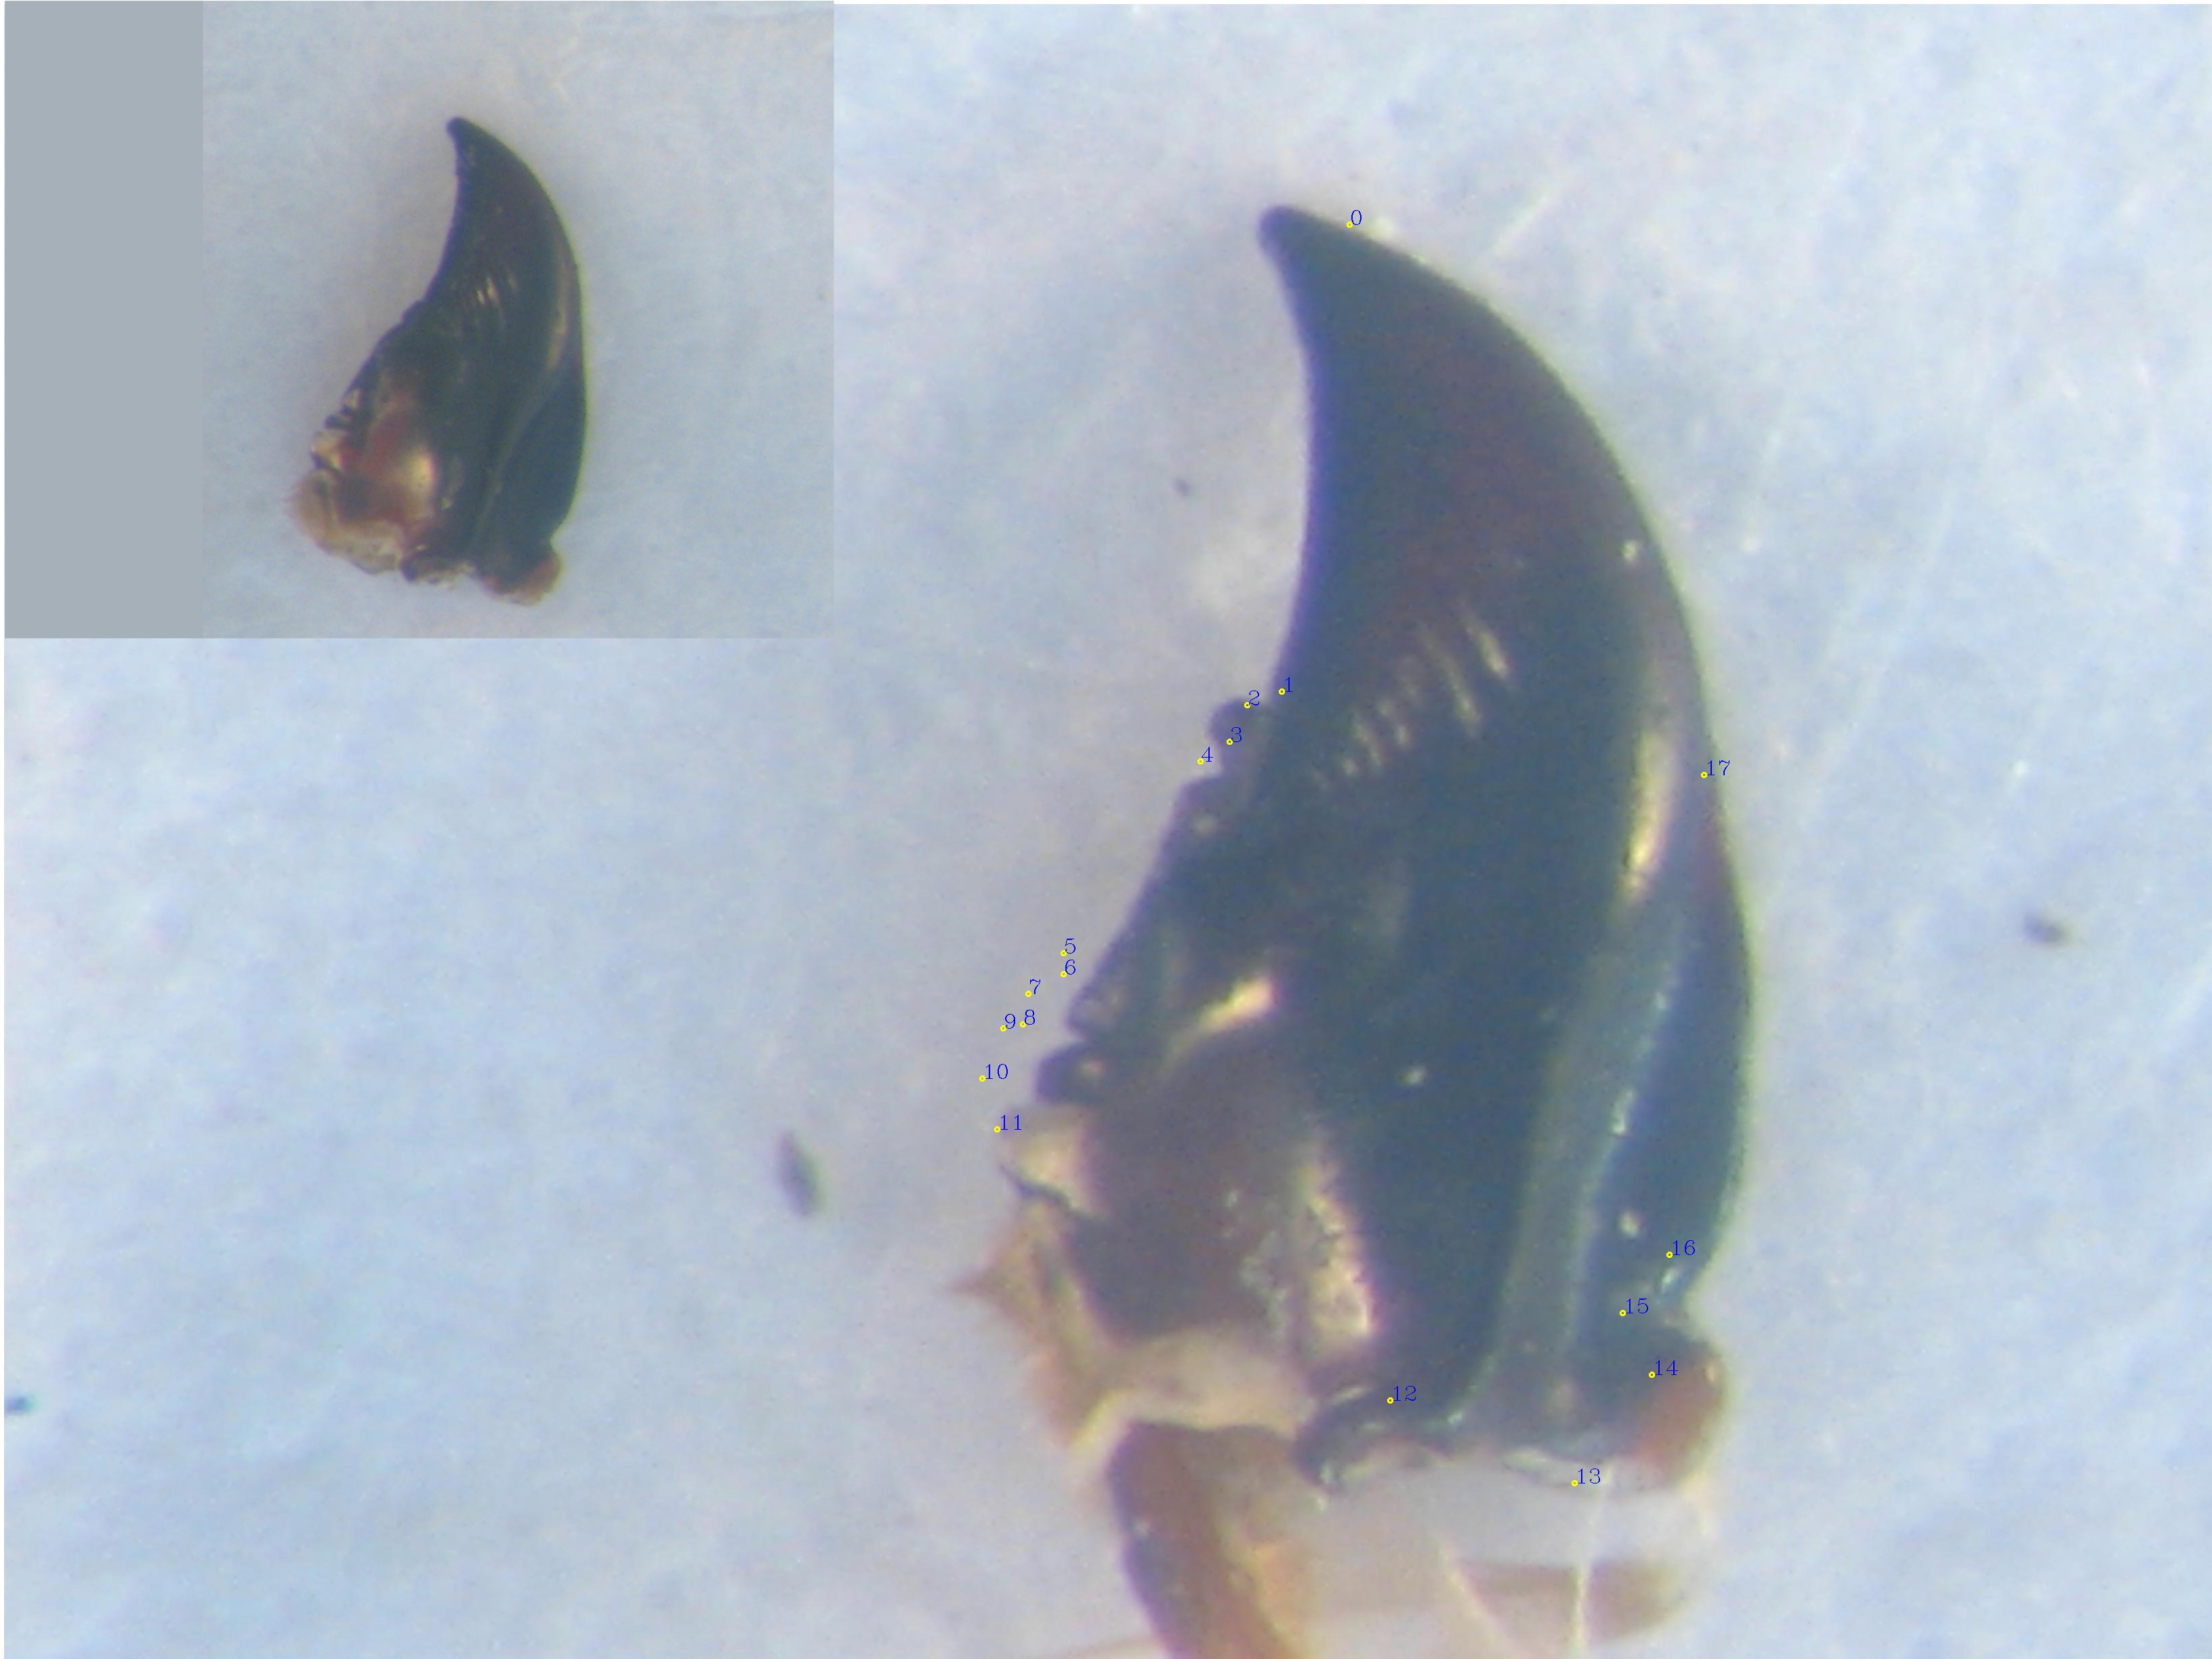
\includegraphics[height=7cm]{images/pht19.JPG}	
	\end{center}
\end{frame}
%%%%%%%%%%%%%%%%%%%%%%%%%%%%%%%%%%%%%%%%%%%%%%%%%%%%%%%%%%%%%%%%%%%%%%%%%%%%%%
\begin{frame}{Method - Template matching}
	\begin{description}
		\item [Purpose:] Refine the estimated landmarks on the scene image 
		\item [Method:] 
			\begin{itemize}
				\item Create a box around each model landmarks on model image
				\item Rotate scene image to match with model
				\item Create a box around each estimated landmarks on scene image
				\item Using Cross-Correlation to refine the estimated landmarks
			\end{itemize}
	\end{description}
\end{frame}
\begin{frame}{Method - Template matching}
	\begin{center}
		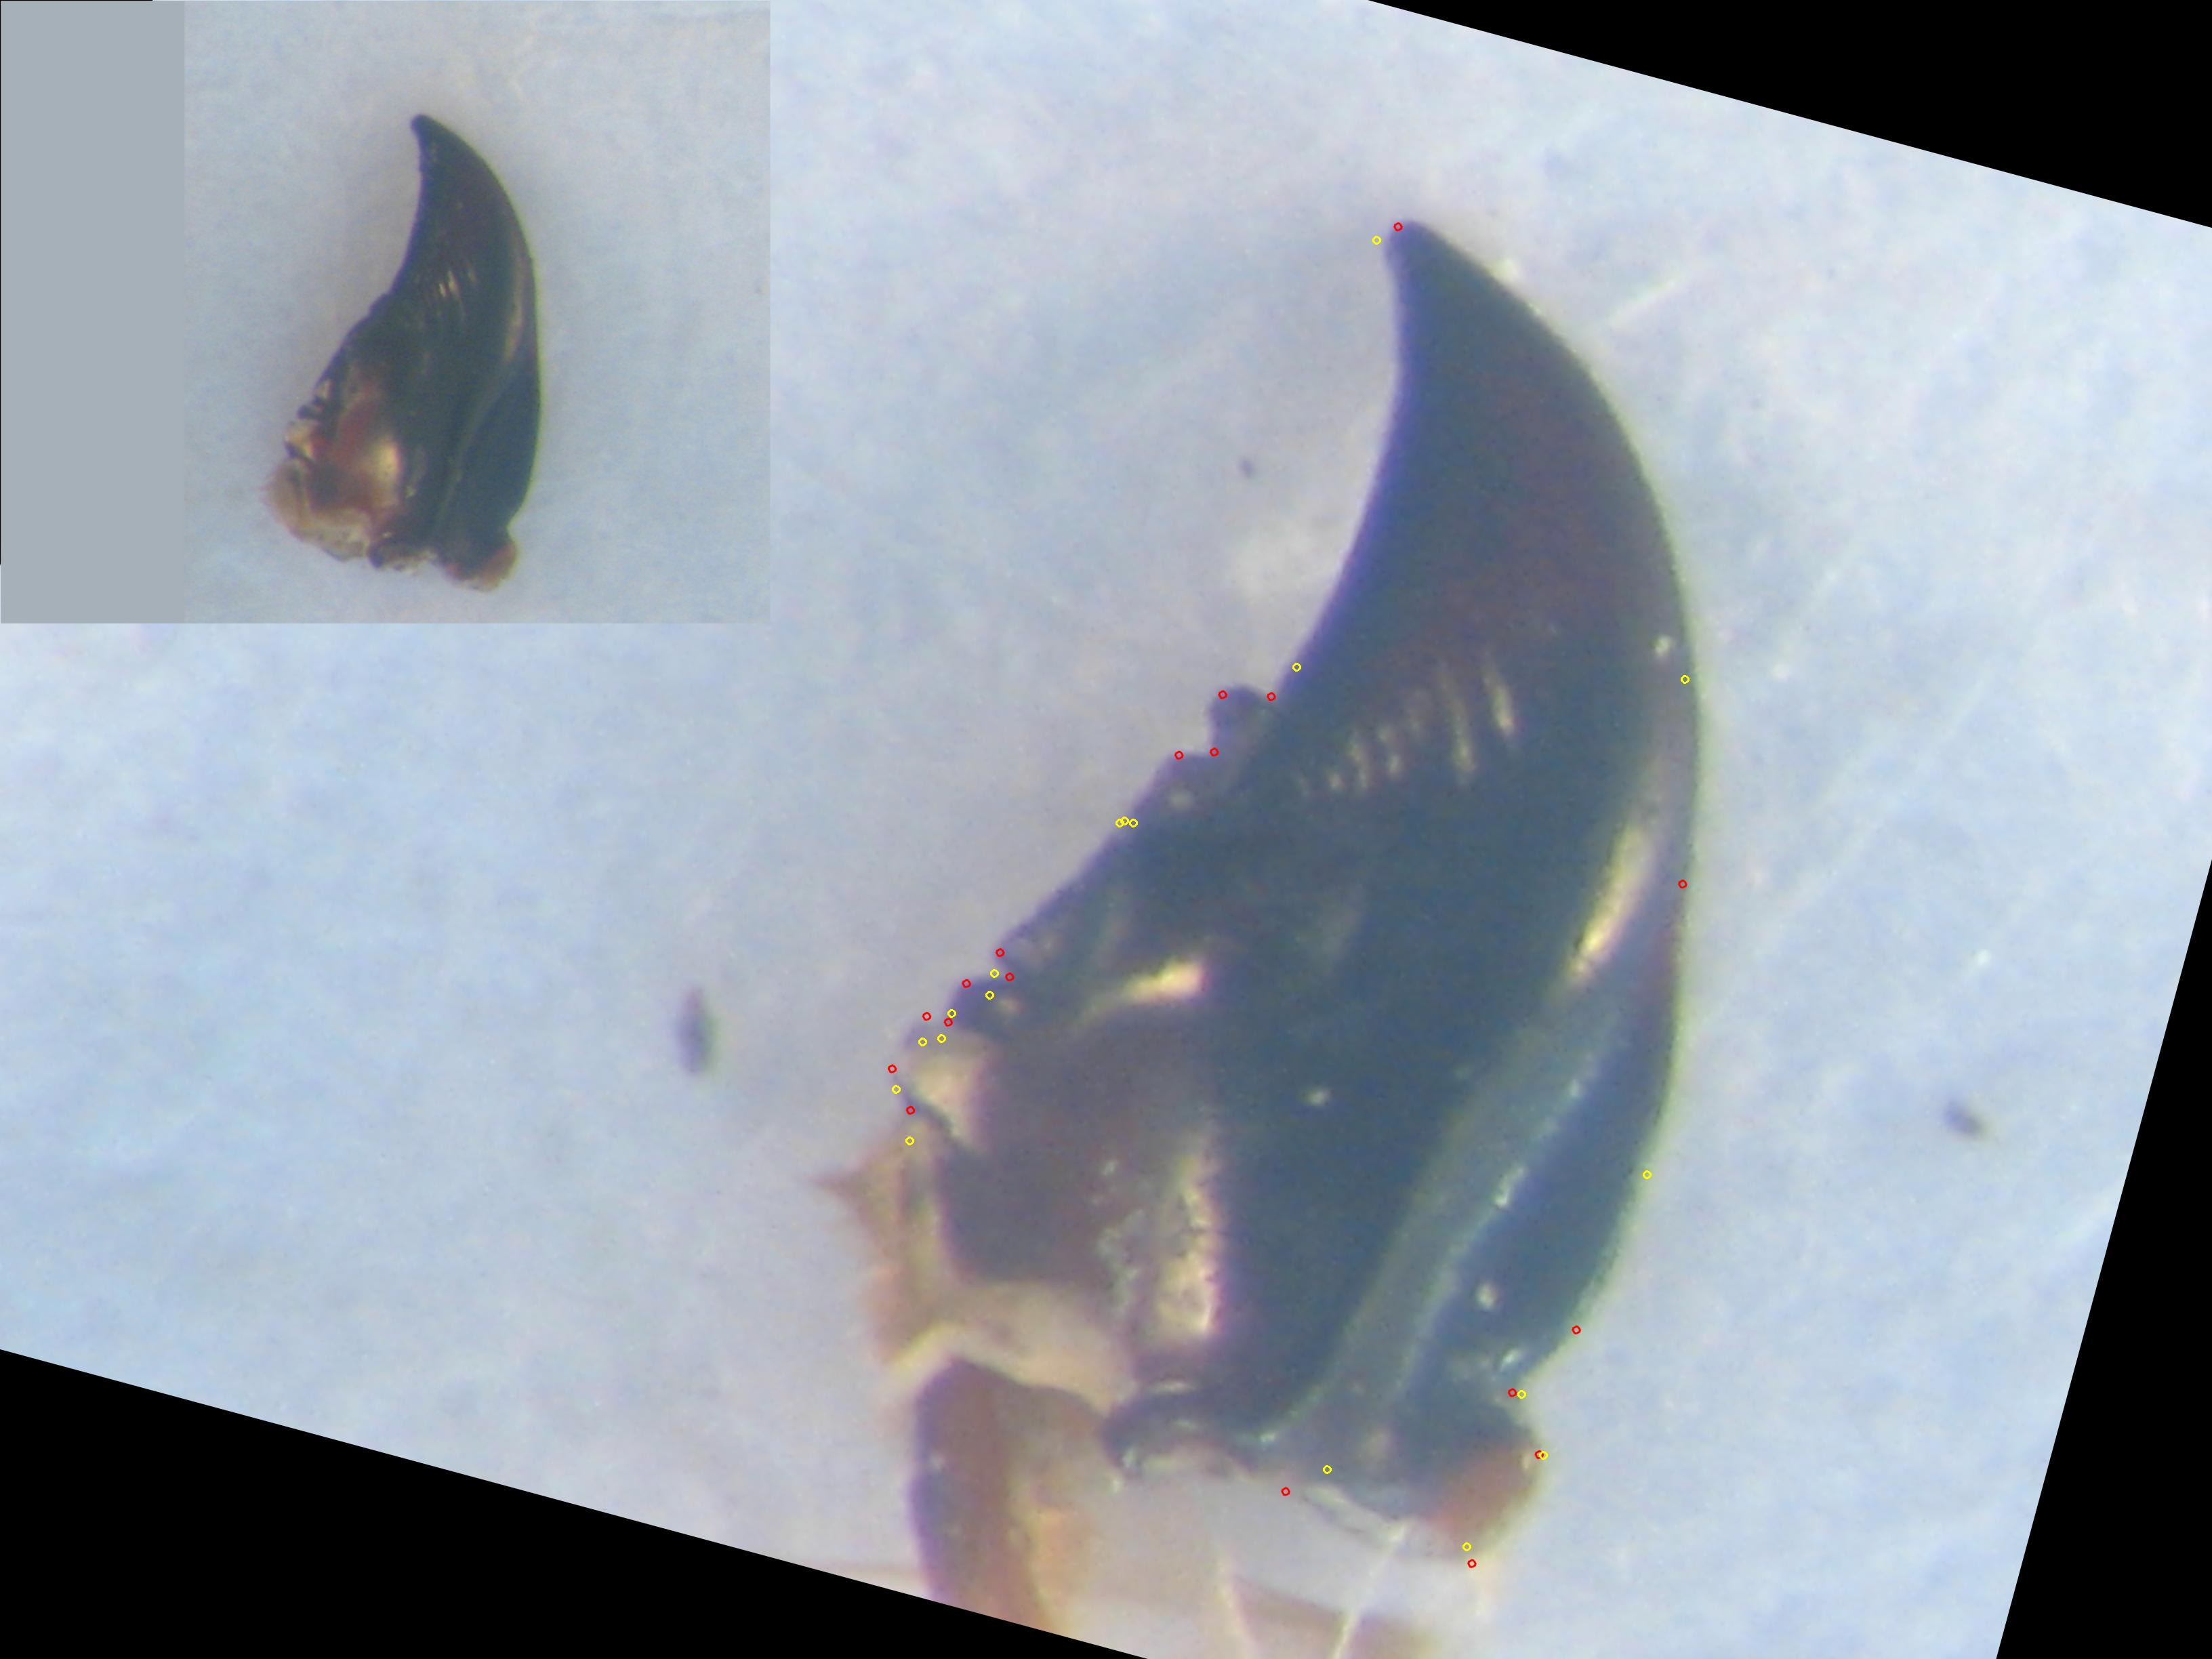
\includegraphics[height=6.5cm]{images/est19.JPG}	
	\end{center}
\end{frame}
%%%%%%%%%%%%%%%%%%%%%%%%%%%%%%%%%%%%%%%%%%%%%%%%%%%%%%%%%%%%%%%%%%%%%%%%%%%%%%
\iffalse
\section{Result}
\begin{frame}{Result}
	\begin{itemize}
	\item Dataset includes 2 set of image (left mandible and right mandible).
	\item Machine 1: Intel(R) Core(TM) 2 Duo CPU T8100 2.1GHz, 2 GB of RAM
	\item Machine 2: Intel(R) Core(TM) i7-4790 CPU 3.6GHz, 16 GB of RAM.
	\end{itemize}	
	\begin{center}
				\begin{tabular}{|p{3cm}|c|c|c|}
					\hline
					Machine & No Of images & Segmentation(second) & Estimation(second) \\ \hline
					Machine 1 & 1 & 0.844 & 31.4245   \\ \hline
					Machine 1 & 290 & 571.576 & 13000.9131   \\ \hline
					Machine 2 & 1 & 0.27782 & 10.4392 \\ \hline
					Machine 2 & 286 & 171.589 & 4665.79 \\ \hline
				\end{tabular}
			\end{center}
\end{frame}
\fi
%%%%%%%%%%%%%%%%%%%%%%%%%%%%%%%%%%%%%%%%%%%%%%%%%%%%%%%%%%%%%%%%%%%%%%%%%%%%%%
\begin{frame}{Result}
	\begin{itemize}
		\item Dataset: \textit{\textcolor{red}{290}} images of right mandible and \textit{\textcolor{red}{286}} images of left mandible.
		\item Landmarks are extracted: \textcolor{red}{18 landmarks} for each \textit{right mandible} and \textcolor{red}{16 landmarks} for each \textit{left mandible}.
	\end{itemize}
\end{frame}
\begin{frame}{Result}
	\begin{center}
		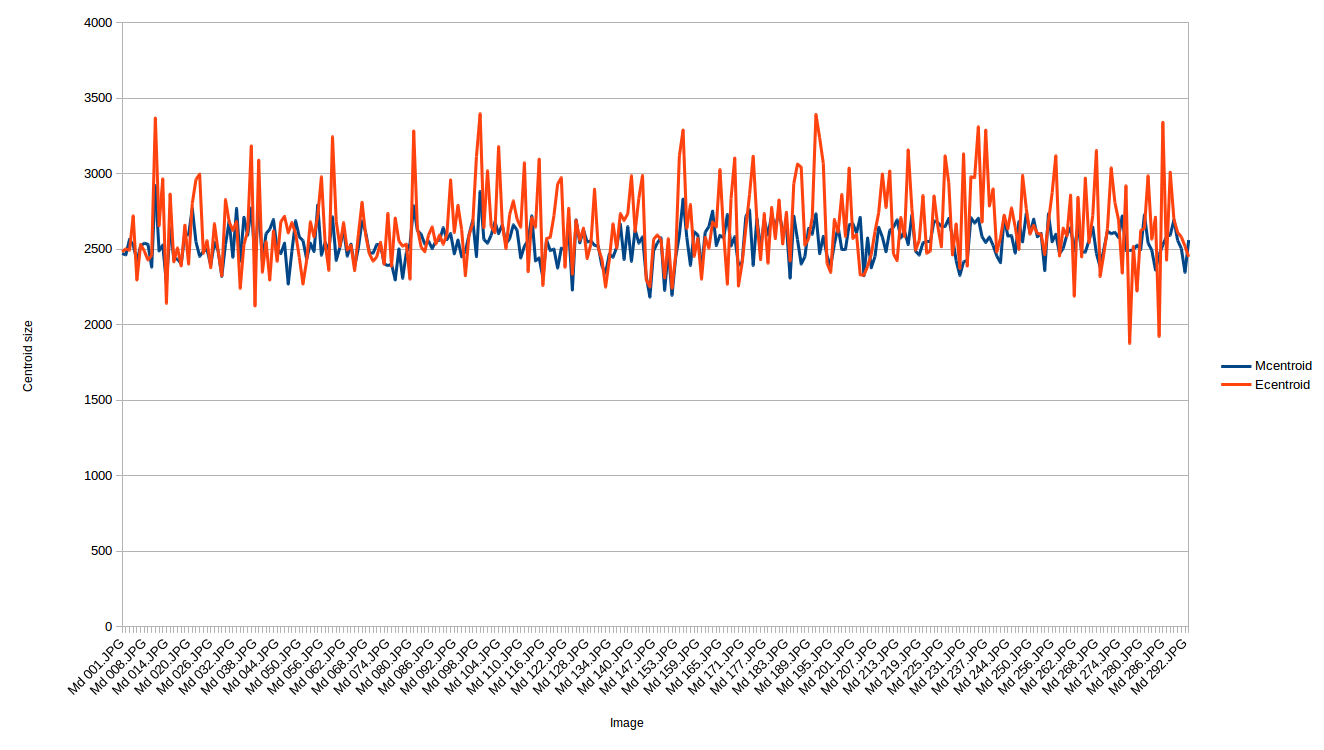
\includegraphics[height=6cm]{images/MdChart.png}	
	\end{center}
\end{frame}
\begin{frame}{Result}
	\begin{center}
		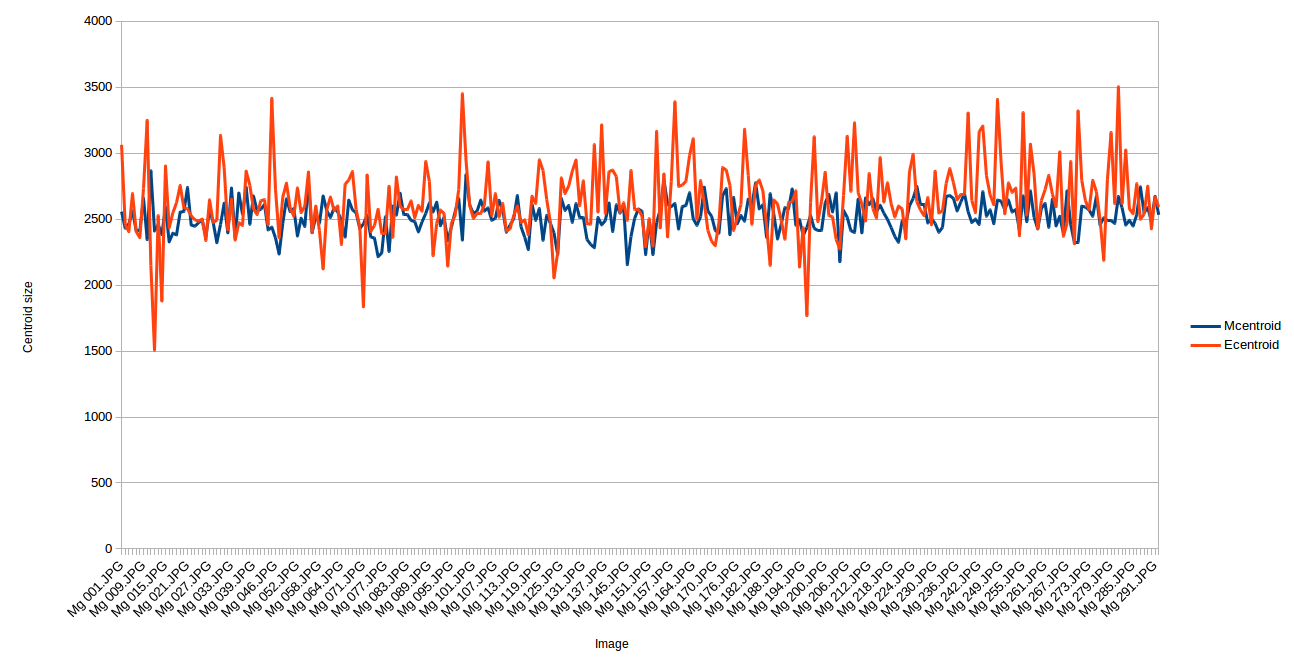
\includegraphics[height=6cm]{images/MgChart.png}	
	\end{center}
\end{frame}
%%%%%%%%%%%%%%%%%%%%%%%%%%%%%%%%%%%%%%%%%%%%%%%%%%%%%%%%%%%%%%%%%%%%%%%%%%%%%%
\section{Conclusion and future works}
\begin{frame}{Conclusion and future works}
	Conclusion:
	\begin{itemize}
		\item This method \textit{(proposed by the article)} can be used to identify the landmarks. But, in some cases, the estimated landmarks are not close with manual landmarks.
		\item Method includes 4 steps. The result of each step can effect to next step.
	\end{itemize}
	Future works:
	\begin{itemize}
		\item Optimize the program based on each process
		\item Apply the method on other datasets: \textit{elytre, head or pronotum}
	\end{itemize}
\end{frame}
\begin{frame}[plain]
  \Huge{\centerline{Thank you !}}
\end{frame}
\end{document}